\documentclass[11pt,a4paper]{article}
\usepackage[T1]{fontenc}
\usepackage[utf8]{inputenc}
\usepackage{lmodern,amsmath,amssymb,amsthm,mathtools}
\usepackage[a4paper,margin=25mm,headheight=15pt,footskip=28pt]{geometry}
\usepackage{microtype,booktabs,tabularx,array,enumitem}
\usepackage{xcolor,tikz,fancyhdr,titlesec,xurl}
\usetikzlibrary{arrows.meta}
\usepackage{hyperref}
\usepackage[nameinlink,noabbrev]{cleveref}

\definecolor{navy}{HTML}{19354D}
\definecolor{teal}{HTML}{126B70}
\definecolor{pale}{HTML}{EDF5F5}
\definecolor{orange}{HTML}{AF551E}
\definecolor{grayink}{HTML}{4B5560}
\hypersetup{colorlinks=true,linkcolor=navy,citecolor=teal,urlcolor=teal,
 pdftitle={H\"older and Zygmund Spectra of the Rvachev--Thue--Morse Operator},
 pdfauthor={OpenAI; prepared for Vladimir Reshetnikov},
 pdfsubject={Exact spectra, finite Fourier reduction, boundary Jordan chains, and sharp decay}}
\urlstyle{same}
\pagestyle{fancy}\fancyhf{}
\fancyhead[L]{\small H\"older and Zygmund spectra}
\fancyhead[R]{\small Finite Fourier reduction}
\fancyfoot[C]{\thepage}
\renewcommand{\headrulewidth}{0.3pt}
\titleformat{\section}{\large\bfseries\color{navy}}{\thesection}{0.7em}{}
\titleformat{\subsection}{\normalsize\bfseries\color{teal}}{\thesubsection}{0.6em}{}
\setlength{\parskip}{3pt plus 1pt}
\setlength{\parindent}{1.1em}
\setlength{\emergencystretch}{2.5em}
\setlist{itemsep=3pt,topsep=4pt,leftmargin=1.6em}
\allowdisplaybreaks
\numberwithin{equation}{section}

\newtheorem{theorem}{Theorem}[section]
\newtheorem{lemma}[theorem]{Lemma}
\newtheorem{proposition}[theorem]{Proposition}
\newtheorem{corollary}[theorem]{Corollary}
\theoremstyle{definition}
\newtheorem{definition}[theorem]{Definition}
\newtheorem{example}[theorem]{Example}
\newtheorem{question}[theorem]{Question}
\theoremstyle{remark}
\newtheorem{remark}[theorem]{Remark}
\newcommand{\C}{\mathbb C}
\newcommand{\R}{\mathbb R}
\newcommand{\Z}{\mathbb Z}
\newcommand{\N}{\mathbb N}
\newcommand{\T}{\mathbb T}
\newcommand{\Pp}{\mathcal P}
\newcommand{\Ll}{\mathcal L}
\newcommand{\Ta}{\mathcal T_a}
\newcommand{\Ub}{\mathcal U_b}
\newcommand{\V}{\mathcal V}
\newcommand{\Id}{I}
\newcommand{\ess}{\mathrm{ess}}
\newcommand{\pt}{\mathrm p}
\newcommand{\Span}{\operatorname{span}}
\newcommand{\dist}{\operatorname{dist}}
\newcommand{\rank}{\operatorname{rank}}
\newcommand{\norm}[1]{\left\lVert#1\right\rVert}
\newcommand{\abs}[1]{\left|#1\right|}
\newcommand{\dd}{\,\mathrm d}
\newcommand{\disk}[1]{\overline{D}(0,#1)}
\newcommand{\openD}[1]{D(0,#1)}
\newcommand{\Gg}[2]{\mathcal G_{#1}(#2)}
\newcommand{\smallspace}{\Lambda_0}
\newcolumntype{Y}{>{\raggedright\arraybackslash}X}

\begin{document}
\hypersetup{pageanchor=false}
\begin{titlepage}
\thispagestyle{empty}
\setlength{\parindent}{0pt}
\vspace*{3mm}
{\sffamily\bfseries\color{teal} PROVEIT RESEARCH EXTENSION\par}
\vspace{6mm}
{\fontsize{29}{34}\selectfont\bfseries\color{navy}
H\"older and Zygmund Spectra\\of the Rvachev--Thue--Morse\\Operator\par}
\vspace{6mm}
{\Large Finite Fourier reduction, critical Jordan chains,\\and optimal decay\par}
\vspace{6mm}
{\large Research manuscript prepared for Vladimir Reshetnikov\par}
{OpenAI\hfill October 2026\par}
\vspace{6mm}
\noindent\fcolorbox{teal}{pale}{\begin{minipage}{0.925\textwidth}
\textbf{Principal conclusion.}
For every $s>0$, on both the periodic H\"older--Zygmund space
$\Lambda^s$ and its little subspace $\smallspace^s$,
\[
 \sigma_{\ess}(\Ll)=\disk{2^{-s-1}},\qquad
 \sigma(\Ll)=\disk{2^{-s-1}}\cup\{1/2,-1/4\}.
\]
The two spaces have different boundary eigenvectors and different boundary
Jordan chains. At $s=1$, both have the sharp residual operator rate
$\Theta(n4^{-n})$, although only the big Zygmund space has actual
length-two Jordan chains at $-1/4$.
\end{minipage}}
\vspace{5mm}
\begin{abstract}
The inspected ProveIt report on integer $C^r$ spectral disks leaves the
noninteger H\"older and Zygmund spectra, the critical $C^1$ eigenspace,
and finite reduction for more general trigonometric masks unresolved.
We give a complete periodic solution for all positive H\"older--Zygmund
orders, together with the noninteger interval extension. The proof uses
an approximation norm in which the operator, modulo a finite Fourier
space, is an exact contraction. This avoids a fractional regularity
bootstrap and identifies every exterior spectral value by a finite matrix.

The argument applies to every nonnegative trigonometric Markov mask for
every integer dilation $b\ge2$. It determines the full Fredholm essential
disk, the point spectrum, all exterior generalized eigenspaces, and the
entire boundary Jordan structure. Each finite-matrix Jordan block on the
critical circle gains one place in the big space; in the little space
the finite-matrix block is unchanged. This yields exact residual power
orders, including the same critical polynomial loss in both spaces.
For the Rvachev operator, the critical classical $C^1$ generalized
eigenspace is exactly two-dimensional and has no nontrivial Jordan chains.
Classical spectral-radius and approximation results are credited explicitly;
publication-level priority is not asserted. All new spectral arguments are
proved here, with finite algebra checked separately by exact arithmetic.
\end{abstract}
\vfill
{\small\color{grayink} Conventional mathematical proofs; no new proof-assistant
formalization is claimed. The ZIP contains the complete source, rendered
article, exact verification program, and source provenance.}
\end{titlepage}

\pagenumbering{roman}
\hypersetup{pageanchor=true}
{\small\setlength{\parskip}{0pt}\tableofcontents}
\clearpage
\pagenumbering{arabic}

\section{The question, the contribution, and the literature}
\label{sec:position}

\subsection{A specific open target in ProveIt}
The Fabius-function branch of ProveIt studies Rvachev's up-function,
Thue--Morse products, and transfer operators arising in Fourier-decay and
mean-square asymptotics. The manuscript \emph{Sharp $C^r$ Spectral Disks
for the Rvachev--Thue--Morse Transfer Operator} proves the integer
$C^r$ spectral formula and then lists several extensions
\cite{repo-cr,repo-index}. Its first research question concerns noninteger
H\"older, little-H\"older, and Zygmund spaces. Its second asks about
the critical $C^1$ eigenvalue $-1/4$, including its multiplicity. Its third
asks for finite Fourier reduction for general trigonometric Markov masks.

This paper resolves the periodic spectral and generalized-eigenvector
parts of those questions. It also proves the noninteger H\"older result
on $[0,1]$, gives exact operator-norm remainder orders, and supplies a
general finite-matrix procedure. The sharp local $C^1$ resolvent problem,
weighted endpoints, and the integer-Zygmund interval problem remain
separate questions. The latter requires more than matching finitely many
endpoint derivatives; \cref{sec:interval} explains the obstruction.

The source snapshot is pinned in \cref{app:provenance}. The earlier
integer $C^r$ result and its elementary three-mode eigenfunctions are
background, not new claims of this paper. Every theorem needed for the
new positive-order approximation-space classification is proved below.

\subsection{What is classical}
The operator is a familiar normalized transfer operator for the
Thue--Morse $g$-function. Baake, Gohlke, Kesseb\"ohmer, and Schindler
identify its invariant measure and study its mixing and scaling
properties \cite{baake}. Weighted dyadic Markov operators, including
weights with zeros, already occur in Conze--Raugi and Hennion
\cite{conze,hennion95}. Hennion's unweighted example also provides a
classical precedent for lacunary eigenfunctions filling a H\"older disk.

Exact essential spectral \emph{radii} on H\"older and Zygmund spaces
have a substantial prior theory. In particular, Baladi--Jiang--Lanford
derive exact formulas on these scales \cite{bjl}; more general Besov
bounds appear in Nakano--Sakamoto \cite{nakano}. Chen--Volkmer study
trigonometric weights, H\"older quasi-compactness, and finite matrices
for growth calculations \cite{chen}. Dutkay's wavelet-Galerkin work is
a related precedent for full continuous-space disks, but its low-pass
normalization is different from the sine mask here \cite{dutkay}.
Uniform trigonometric approximation and Jackson--Stechkin inequalities
are likewise classical \cite{foucart,devore}.

The contribution made here is a complete and elementary resolution of
the stated repository questions: an exact quotient contraction, the full
spectral set rather than only its radius, a finite core for every finite
Markov mask, the big/little boundary classification, the critical Jordan
extension, and sharp residual power orders. The reviewed sources establish
important antecedents; the present literature check does not certify that
every specialization is new to the worldwide literature.

\begin{center}
\small
\begin{tabularx}{\textwidth}{@{}p{0.27\textwidth}Y Y@{}}
\toprule
Target & Result here & Remaining limitation\\
\midrule
Noninteger H\"older spectra & Exact spectrum, essential spectrum, and point
spectrum on circle and interval & Endpoint-weighted variants remain open\\
Periodic Zygmund spectra & All $s>0$, including integer orders & No integer
interval-Zygmund theorem is inferred\\
Critical $C^1$ eigenspace & Exactly two-dimensional; all generalized vectors
are ordinary eigenvectors & Sharp local $C^1$ resolvent growth is not settled\\
Finite trigonometric masks & Explicit core matrix, boundary Jordan theorem,
and exact residual orders & Positivity and finite Fourier support are hypotheses\\
\bottomrule
\end{tabularx}
\end{center}

\section{Spaces, normalization, and the principal theorem}
\label{sec:main}

\subsection{The operator}
Write $\T=\R/\Z$ and use complex-valued functions. The repository
normalization is
\begin{equation}
 (\Ll f)(x)=\frac12\left[
 \sin^2\!\left(\frac{\pi x}{2}\right)f(x/2)
 +\cos^2\!\left(\frac{\pi x}{2}\right)f((x+1)/2)
 \right].
 \label{eq:L}
\end{equation}
We first work with the Markov normalization
\begin{equation}
 \Pp=2\Ll,\qquad \Pp1=1,\qquad
 \norm{\Pp f}_\infty\le\norm f_\infty.
 \label{eq:P}
\end{equation}
The two branch terms interchange when $x$ is replaced by $x+1$, so their
sum is periodic. Every final spectral value for $\Pp$ is divided by two
to obtain the corresponding value for $\Ll$.

\subsection{Big and little regularity}
Let $e_m(x)=\exp(2\pi i m x)$ and
\begin{equation}
 \V_N=\Span\{e_m:|m|\le N\},\qquad
 E_N(f)=\inf_{p\in\V_N}\norm{f-p}_\infty
 \quad(N\ge0).
 \label{eq:approx}
\end{equation}
For $s>0$, define the periodic H\"older--Zygmund space by the equivalent
approximation norm
\begin{equation}
 \Lambda^s=\left\{f\in C(\T):
 \norm f_{\Lambda^s}:=\norm f_\infty+
 \sup_{N\ge1}N^sE_N(f)<\infty\right\}.
 \label{eq:big}
\end{equation}
Its little subspace is
\begin{equation}
 \smallspace^s=\left\{f\in\Lambda^s:N^sE_N(f)\longrightarrow0\right\}.
 \label{eq:little}
\end{equation}
It is precisely the closure of trigonometric polynomials, equivalently
of smooth periodic functions, in $\Lambda^s$.

For $s=r+\alpha$, $r\ge0$ an integer and $0<\alpha<1$, these are the
usual spaces $C^{r,\alpha}(\T)$ and $h^{r,\alpha}(\T)$, with equivalent
norms. At $s=m\in\N$, $\Lambda^m$ is the Zygmund space
$B^m_{\infty,\infty}$, and $\smallspace^m$ is its little subspace.
In particular, $\Lambda^1$ is defined equivalently by bounded symmetric
second differences divided by $|h|$. It is not the Lipschitz space and
not $C^1$. One has
\begin{equation}
 C^m(\T)\subseteq\smallspace^m(\T)\subseteq\Lambda^m(\T).
 \label{eq:Cr-inclusion}
\end{equation}
The approximation characterizations and these identifications are proved
in \cref{app:approximation}; they are not additional spectral assumptions.

\subsection{Spectral terminology}
We use the Fredholm essential spectrum
\[
 \sigma_{\ess}(T)=\{z\in\C:T-zI\text{ is not Fredholm}\}.
\]
The point spectrum is $\sigma_{\pt}(T)=\{z:\ker(T-zI)\ne0\}$. Write
\begin{equation}
 \Gg{z}{T}=\bigcup_{k\ge1}\ker(T-zI)^k
 \label{eq:rootspace}
\end{equation}
for the algebraic generalized eigenspace. At a nonisolated spectral
point we speak directly about this space and its Jordan chains; we do
not assign a Riesz projection there.

\begin{theorem}[Complete periodic spectral classification]
\label{thm:sine-main}
For every $s>0$, put $\rho_s=2^{-s-1}$. On both $\Lambda^s$ and
$\smallspace^s$,
\begin{equation}
 \sigma_{\ess}(\Ll)=\disk{\rho_s},\qquad
 \sigma(\Ll)=\disk{\rho_s}\cup\{1/2,-1/4\}.
 \label{eq:sine-spectrum}
\end{equation}
The point spectra are
\begin{align}
 \sigma_{\pt}(\Ll;\Lambda^s)
 &=\disk{\rho_s}\cup\{1/2,-1/4\},\label{eq:big-point}\\
 \sigma_{\pt}(\Ll;\smallspace^s)
 &=\openD{\rho_s}\cup\{1/2,-1/4\}.
 \label{eq:little-point}
\end{align}
Every point of the closed disk in the big space, and of the open disk in
the little space, has infinite geometric multiplicity.

The eigenvalue $1/2$ is isolated and simple for all $s>0$.
The eigenvalue $-1/4$ is isolated exactly when $s>1$; there it is
semisimple with two-dimensional eigenspace
\begin{equation}
 H=\Span\{\sin(2\pi x),\ \cos(2\pi x)+1/3\}.
 \label{eq:H}
\end{equation}
Every exterior generalized eigenvector belongs to
$F_1=\Span\{e_{-1},1,e_1\}$.
\end{theorem}

\begin{theorem}[The critical Jordan transition]
\label{thm:sine-jordan}
Let $N=\Ll+\tfrac14 I$.
On the big Zygmund space $\Lambda^1$,
\begin{equation}
 \Gg{-1/4}{\Ll}=\ker N^2,\qquad
 \dim\bigl(\ker N^2/\ker N\bigr)=2,
 \label{eq:critical-big}
\end{equation}
while $\ker N$ is infinite-dimensional. There are two independent
length-two Jordan chains and no chain of length three.
On $\smallspace^1$, and also on classical $C^1(\T)$,
\begin{equation}
 \Gg{-1/4}{\Ll}=\ker N=H.
 \label{eq:critical-little}
\end{equation}
All other boundary generalized eigenvectors in a big $\Lambda^s$ are
ordinary eigenvectors. In a little space, the only possible boundary
generalized vectors are the finite-core ones; for noninteger $s$ there
are none.
\end{theorem}

The same noninteger H\"older statements hold on $[0,1]$. The critical
$C^1$ statement also holds on $[0,1]$. Integer Zygmund statements in this
paper are periodic statements.

\begin{figure}[ht]
\centering
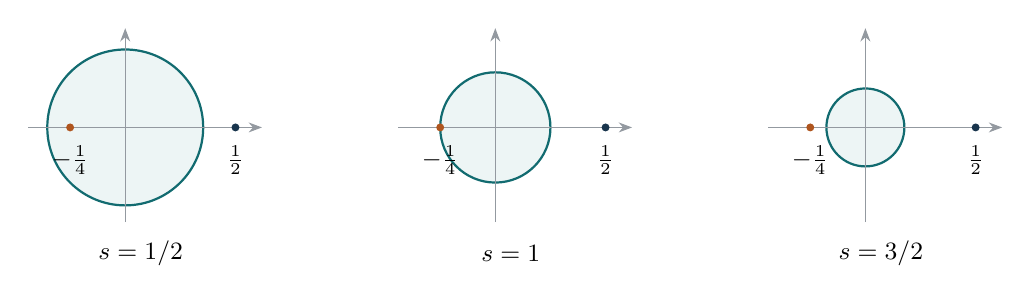
\begin{tikzpicture}[x=2.8cm,y=2.8cm,>=Stealth,font=\small]
\foreach \c/\s/\rad/\lab in {0/0.5/0.353553/{s=1/2},4.7/1/0.25/{s=1},9.4/1.5/0.176777/{s=3/2}} {
 \begin{scope}[xshift=\c cm]
  \fill[pale] (0,0) circle (\rad);
  \draw[teal,thick] (0,0) circle (\rad);
  \draw[grayink!60,->] (-0.44,0)--(0.62,0);
  \draw[grayink!60,->] (0,-0.43)--(0,0.45);
  \fill[navy] (0.5,0) circle (0.018);
  \fill[orange] (-0.25,0) circle (0.018);
  \node[below=3pt] at (0.5,0) {$\frac12$};
  \node[below=3pt] at (-0.25,0) {$-\frac14$};
  \node at (0.07,-0.57) {$\lab$};
 \end{scope}
}
\end{tikzpicture}
\caption{The spectrum of $\Ll$ as regularity increases. The essential
disk has radius $2^{-s-1}$. The same spectral set occurs in the big and
little spaces, but their boundary eigenspaces differ. At $s=1$, $-1/4$
meets the essential circle and the big Zygmund Jordan extension appears.}
\label{fig:disks}
\end{figure}

\section{An exact finite Fourier reduction for every finite Markov mask}
\label{sec:finite-core}

\subsection{The general operator}
Fix an integer $b\ge2$ and a real, nonnegative trigonometric polynomial
\begin{equation}
 a(x)=\sum_{|j|\le d}a_j e_j(x)
 \quad\text{such that}\quad
 \frac1b\sum_{\ell=0}^{b-1}a((x+\ell)/b)=1.
 \label{eq:mask}
\end{equation}
We set $a_j=0$ for $|j|>d$. The constant mask has $d=0$; otherwise
$d$ can be its exact degree.
Define
\begin{equation}
 (\Ta f)(x)=\frac1b\sum_{\ell=0}^{b-1}
 a((x+\ell)/b)f((x+\ell)/b),\qquad
 (\Ub f)(x)=f(bx).
 \label{eq:general-transfer}
\end{equation}
The Markov condition is equivalent to $a_0=1$ and $a_{bj}=0$ for every
nonzero integer $j$. Nonnegativity and the normalization imply
\begin{equation}
 \norm{\Ta f}_\infty\le\norm f_\infty,
 \qquad \Ta\Ub=I.
 \label{eq:contraction-rightinverse}
\end{equation}
For the Rvachev operator, $b=2$ and $a(x)=1-\cos(2\pi x)$, so
$\Ta=\Pp$.

\begin{lemma}[Fourier rule and invariant core]
\label{lem:fourier}
For each integer $m$,
\begin{equation}
 \Ta e_m=\sum_{\substack{|j|\le d\\b\mid m+j}}
 a_j e_{(m+j)/b},\qquad
 \Ta\V_N\subseteq\V_{\lfloor(N+d)/b\rfloor}.
 \label{eq:fourier-general}
\end{equation}
Put
\begin{equation}
 \xi=\frac d{b-1},\qquad K=\lfloor\xi\rfloor,\qquad F=\V_K.
 \label{eq:core-size}
\end{equation}
Then $F$ is invariant, and the matrix of $A=\Ta|_F$ in the Fourier
basis indexed by $-K,\ldots,K$ is
\begin{equation}
 A_{k,m}=a_{bk-m}.
 \label{eq:matrix}
\end{equation}
\end{lemma}
\begin{proof}
Insert $a$ and $e_m$ into \eqref{eq:general-transfer}. The finite sum
$b^{-1}\sum_{\ell=0}^{b-1}\exp(2\pi i(m+j)\ell/b)$ is one when
$b\mid m+j$ and zero otherwise. This proves the Fourier rule and the
degree bound. Write $d=(b-1)K+r$ with $0\le r\le b-2$; then
$\lfloor(K+d)/b\rfloor=K$. The coefficient at $e_k$ in the image of
$e_m$ is $a_{bk-m}$.
\end{proof}

\subsection{The shifted approximation norm}
For an integer $N\ge K$ set
\begin{equation}
 v_N=N+1-\xi>0,
 \qquad q_s(f)=\sup_{N\ge K}v_N^s E_N(f).
 \label{eq:shifted-seminorm}
\end{equation}
Since $v_N\asymp N$ for large $N$, the norm
$\norm f_\infty+q_s(f)$ defines the same $\Lambda^s$ as
\eqref{eq:big}. The little condition is equivalently
$v_N^sE_N(f)\to0$.

The seminorm $q_s$ vanishes precisely on $F$. It is unchanged by adding
an element of $F$, and it gives a complete norm on the quotient
$\Lambda^s/F$. Indeed, the quotient norm induced by
$\norm f_\infty+q_s(f)$ equals
\begin{equation}
 E_K(f)+q_s(f),\qquad
 E_K(f)\le v_K^{-s}q_s(f),
 \label{eq:quotient-norm}
\end{equation}
so the two quotient norms are equivalent. The same reasoning applies to
the little space.

\begin{theorem}[Exact contraction after removal of the finite core]
\label{thm:quotient}
For $N\ge K$ and $n\ge0$, define the integer
\begin{equation}
 \nu_n(N)=b^n(N+1)-d\sum_{j=0}^{n-1}b^j-1.
 \label{eq:index}
\end{equation}
Then
\begin{gather}
 v_{\nu_n(N)}=b^n v_N,\qquad
 \Ta^n\V_{\nu_n(N)}\subseteq\V_N,\label{eq:index-properties}\\
 E_N(\Ta^n f)\le E_{\nu_n(N)}(f),\qquad
 q_s(\Ta^n f)\le b^{-ns}q_s(f).
 \label{eq:exact-contraction}
\end{gather}
Thus the operator $Q$ induced on either quotient by $F$ satisfies
$\norm{Q^n}\le b^{-ns}$ in the norm $q_s$.
For every fixed $f\in\smallspace^s$ one has the stronger statement
\begin{equation}
 b^{ns}q_s(\Ta^n f)\longrightarrow0.
 \label{eq:little-strong}
\end{equation}
\end{theorem}
\begin{proof}
The affine map $\nu_1(N)=b(N+1)-d-1$ has $\nu_1(N)\ge N$ for
$N\ge K$, because its minimum increment is $b-1-r\ge1$ in the
notation of \cref{lem:fourier}. Also
\[
 \left\lfloor\frac{\nu_1(N)+d}{b}\right\rfloor
 =\left\lfloor N+1-\frac1b\right\rfloor=N.
\]
Iteration gives \eqref{eq:index} and the degree inclusion. The identity
for $v$ follows from $d=(b-1)\xi$.

Choose a polynomial $p$ of degree at most $\nu_n(N)$. Its image has
degree at most $N$, and the Markov contraction gives
$E_N(\Ta^n f)\le\norm{\Ta^n(f-p)}_\infty\le\norm{f-p}_\infty$.
Taking the infimum proves the first inequality in
\eqref{eq:exact-contraction}; multiplying by $v_N^s$ and taking the
supremum proves the second. Finally,
\[
 b^{ns}q_s(\Ta^n f)
 \le\sup_{M\ge\nu_n(K)}v_M^sE_M(f),
\]
and $\nu_n(K)\to\infty$. The right side tends to zero in the little
space.
\end{proof}

For the sine mask, $\xi=K=1$, $v_N=N$, and $\nu_n(N)=2^nN$.
The entire mechanism then reduces to
\begin{equation}
 \boxed{\ E_N(\Pp^n f)\le E_{2^nN}(f).\ }
 \label{eq:sine-contraction}
\end{equation}
This is why a finite Fourier calculation can determine all exterior
spectral values without assuming that their eigenvectors are analytic or
bootstrapping them through fractional derivatives.

\section{The full disk and the finite exterior spectrum}
\label{sec:spectrum}

\subsection{Polynomial defects and lacunary series}
The right inverse in \eqref{eq:contraction-rightinverse} makes an
infinite-dimensional defect space explicit. For every integer $m$ not
divisible by $b$, put
\begin{equation}
 h_m=e_m-\Ub\Ta e_m.
 \label{eq:polynomial-defect}
\end{equation}
Then $h_m$ is a trigonometric polynomial and $\Ta h_m=0$. All frequencies
of $\Ub\Ta e_m$ are divisible by $b$. The coefficient of $h_m$ at a
nonmultiple $m'$ of $b$ is therefore $\delta_{m,m'}$. Thus these defects
are linearly independent.

For a polynomial $h$ and $|z|<1$, define the uniformly convergent series
\begin{equation}
 W_z(h)=\sum_{n=0}^\infty z^n\Ub^n h.
 \label{eq:W}
\end{equation}
We shall use it both for kernel defects and for finite-core vectors.

\begin{lemma}[Regularity and the exact series identity]
\label{lem:W}
Let $s>0$ and $\rho=b^{-s}$.
If $h$ is a polynomial, then $W_z(h)\in\Lambda^s$ for $|z|=\rho$,
and $W_z(h)\in\smallspace^s$ for $|z|<\rho$.
For every $|z|<1$,
\begin{equation}
 (\Ta-zI)W_z(h)=\Ta h,
 \qquad (I-z\Ub)W_z(h)=h.
 \label{eq:W-identities}
\end{equation}
At $|z|=\rho$ the partial sums are uniformly bounded in $\Lambda^s$.
\end{lemma}
\begin{proof}
Suppose first that $h$ has degree $D\ge1$. A partial sum through index
$j$ has degree at most $Db^j$. For $N\ge D$, let $j$ be the largest
integer with $Db^j\le N$. The remaining uniform tail is at most
\[
 \norm h_\infty\frac{|z|^{j+1}}{1-|z|}.
\]
When $|z|=b^{-s}$, the inequality $N<Db^{j+1}$ bounds this tail by
$C_{s,h}N^{-s}$. The same estimate, with an earlier stopping point
when necessary, applies uniformly to every finite partial sum.
Constant polynomials cause no difficulty because their entire series
is constant.

If $0<|z|<b^{-s}$, choose $t>s$ with $|z|<b^{-t}$. The same argument,
or absolute convergence in the $\Lambda^s$ norm, gives membership in
$\smallspace^s$. More explicitly,
$\norm{\Ub^n h}_{\Lambda^s}\le C_{s,h}b^{ns}$; the series converges
in that norm and each term is smooth. The case $z=0$ is immediate.

Both identities follow by uniformly convergent summation and
$\Ta\Ub^n=\Ub^{n-1}$ for $n\ge1$.
\end{proof}

\begin{remark}[The topology of boundary convergence]
The boundary series is proved to converge uniformly and to belong to
the big space. It is generally not a convergent series in the big
H\"older--Zygmund norm. Confusing these two assertions would incorrectly
put the boundary eigenfunctions in the little space.
\end{remark}

\begin{theorem}[General finite-mask spectrum]
\label{thm:general-spectrum}
Under \eqref{eq:mask}, let $A$ be \eqref{eq:matrix} and
$\rho=b^{-s}$, $s>0$. On both $\Lambda^s$ and $\smallspace^s$,
\begin{equation}
 \sigma_{\ess}(\Ta)=\disk\rho,
 \qquad \sigma(\Ta)=\disk\rho\cup\sigma(A).
 \label{eq:general-spectrum}
\end{equation}
Furthermore,
\begin{align}
 \sigma_{\pt}(\Ta;\Lambda^s)&=\disk\rho\cup\sigma(A),\\
 \sigma_{\pt}(\Ta;\smallspace^s)&=\openD\rho\cup\sigma(A).
 \label{eq:general-points}
\end{align}
Every point of the closed disk in the big space, and of the open disk
in the little space, has infinite geometric multiplicity. For
$|z|>\rho$, on either space,
\begin{equation}
 \Gg z{\Ta}=\Gg zA\subseteq F.
 \label{eq:exterior-roots}
\end{equation}
The same root-space equality holds at $|z|=\rho$ on the little space.
\end{theorem}

\begin{proof}
Choose a bounded linear complement to the finite-dimensional invariant
space $F$. The quotient norm $q_s$ identifies the operator with a
bounded upper triangular block operator
\begin{equation}
 \Ta=\begin{pmatrix}A&B\\0&Q\end{pmatrix},
 \qquad \norm{Q^n}\le\rho^n.
 \label{eq:blocks}
\end{equation}
Such a complement exists because a finite-dimensional subspace of a
Banach space is complemented. Its second block is identified with the
quotient, so the displayed power bound is valid in an equivalent norm.

For $|z|>\rho$, $Q-zI$ is invertible by its Neumann series. Elementary
block inversion then shows that $\Ta-zI$ is invertible if and only if
$A-zI$ is invertible. Projecting a generalized eigenvector to the
quotient also proves \eqref{eq:exterior-roots}. Even when $A-zI$ is
singular, the full block operator is Fredholm of index zero: multiply
by invertible triangular factors to remove $B$, leaving a finite matrix
and an invertible infinite block.

For every polynomial kernel defect $h$, \cref{lem:W} gives
$\Ta W_z(h)=zW_z(h)$ at every $|z|\le\rho$ in the big space and every
$|z|<\rho$ in the little space. The second identity in
\eqref{eq:W-identities} makes $h\mapsto W_z(h)$ injective.
Thus all interior points have infinite-dimensional kernels, so they are
not Fredholm. The set of non-Fredholm operators is closed; hence the
whole closed disk is essential. The exterior Fredholm statement proves
that there are no further essential points. Every eigenvalue of $A$
has a polynomial eigenvector in both spaces. This proves the spectral
sets and the big-space point spectrum.

It remains to exclude extra little-space boundary eigenvectors and
generalized vectors. Let $f$ be generalized at $|z|=\rho$, and write
$y$ for its quotient class. If $y\ne0$, let $k$ be its Jordan height,
so $(Q-zI)^ky=0$ and $(Q-zI)^{k-1}y\ne0$. Then
\begin{equation}
 z^{-n}Q^ny
 =\sum_{j=0}^{k-1}\binom nj z^{-j}(Q-zI)^jy.
 \label{eq:jordan-growth}
\end{equation}
The right side is a nonzero vector-valued polynomial, of degree $k-1$.
It cannot tend to zero. But \eqref{eq:little-strong} says precisely
that its norm tends to zero in the little quotient. Thus $y=0$ and
$f\in F$. This proves the boundary root-space statement and completes
\eqref{eq:general-points}.
\end{proof}

\subsection{Two useful consequences}
For each compact operator $C$ on either regularity space and every
$n\ge1$,
\begin{equation}
 \norm{\Ta^n-C}\ge\rho^n.
 \label{eq:compact-lower}
\end{equation}
Indeed, the spectrum of the Calkin image of $\Ta$ is the Fredholm
essential disk. Spectral mapping puts a disk of radius $\rho^n$ in the
spectrum of its $n$th power, and the quotient norm dominates spectral
radius. Equivalently, \eqref{eq:compact-lower} is the unavoidable
exponential obstruction to approximation by compact operators.

There is also a precise regularity obstruction. If $\Ta f=zf$,
$f\notin F$, and $f$ is continuous, then exact degree collapse and
Markov contraction give
\begin{equation}
 E_{\nu_n(K)}(f)\ge |z|^n E_K(f).
 \label{eq:sharp-approx-lower}
\end{equation}
Thus a noncore eigenvector at $|z|=b^{-s}$ cannot have little order
$s$, or any higher H\"older--Zygmund regularity. For a quotient
Jordan chain of height $k$, the same argument and
\eqref{eq:jordan-growth} give the lower bound
$c n^{k-1}|z|^n$ along this approximation sequence. A longer quotient
chain would require a logarithmic loss in approximation order.

\section{Every boundary Jordan chain is determined by the finite core}
\label{sec:jordan}

\begin{theorem}[Boundary extension by one Jordan level]
\label{thm:general-jordan}
Assume \eqref{eq:mask}, fix $s>0$, and let $|z|=\rho=b^{-s}$.
On the big space $\Lambda^s$, put $N=\Ta-zI$. For every $j\ge1$,
the map induced by $N$ is an isomorphism
\begin{equation}
 \frac{\ker N^{j+1}}{\ker N}
 \xrightarrow{\ \cong\ }\ker(A-zI)^j.
 \label{eq:root-quotients}
\end{equation}
In particular,
\begin{equation}
 \frac{\Gg z{\Ta}}{\ker(\Ta-zI)}\cong\Gg zA.
 \label{eq:root-quotient-full}
\end{equation}
If $z$ is not an eigenvalue of $A$, all its generalized vectors are
ordinary eigenvectors. If the largest Jordan block of $A$ at $z$ has
length $\ell\ge1$, the largest Jordan chain in the big space has
length exactly $\ell+1$. Each finite-core block gains one place;
the remaining boundary eigenvectors have no further generalized level.

On the little space,
$\Gg z{\Ta}=\Gg zA$, so all finite-core Jordan lengths are unchanged.
\end{theorem}

\begin{proof}
Let $f$ be any generalized vector in the big space and project it to
the quotient. Formula \eqref{eq:jordan-growth}, together with
$\norm{Q^n}\le\rho^n$, shows that the quotient Jordan height is at
most one. Therefore $Nf\in F$. It is itself generalized at $z$, so
$Nf\in\Gg zA$. For $f\in\ker N^{j+1}$ this gives
$Nf\in\ker(A-zI)^j$. The kernel of the induced map is exactly
$\ker N$.

To prove surjectivity, take $h\in\Gg zA$. Since $z\ne0$, $A$ is
invertible on this finite generalized eigenspace. Set
\begin{equation}
 v=(A|_{\Gg zA})^{-1}h,\qquad
 R_z h=W_z(v)=\sum_{n=0}^\infty z^n\Ub^n v.
 \label{eq:right-lift}
\end{equation}
The vector $v$ is a polynomial. By \cref{lem:W}, $R_zh$ belongs to
the big space and
\begin{equation}
 (\Ta-zI)R_zh=\Ta v=Av=h.
 \label{eq:lift-identity}
\end{equation}
If $(A-zI)^jh=0$, then $N^{j+1}R_zh=0$. This proves surjectivity
in \eqref{eq:root-quotients} and hence all quotient identities.

For the maximal length, $Nf\in\Gg zA$ implies
$N^{\ell+1}f=0$ for every generalized $f$. Choosing $h$ of core Jordan
height $\ell$ in \eqref{eq:right-lift} produces a vector of height
$\ell+1$. More precisely, the dimensions in
\eqref{eq:root-quotients} are the sums of $\min(j,m)$ over the core
block lengths $m$, which are exactly the dimensions obtained by
increasing each such block length by one. The eigenspace itself is
infinite-dimensional. The little-space assertion was established in
\cref{thm:general-spectrum}.
\end{proof}

The theorem describes an embedded boundary phenomenon. Its statement
does not depend on isolation of the spectral point, and it does not
introduce a spectral projection on the essential circle.

\begin{proposition}[Interior chains of arbitrary finite length]
\label{prop:interior-chains}
At each $|z|<b^{-s}$, both spaces contain Jordan chains of every finite
length, with infinitely many independent bottom eigenvectors.
\end{proposition}
\begin{proof}
For a polynomial kernel seed $h$, the series $W_z(h)$ is norm-holomorphic
in $|z|<b^{-s}$, because its differentiated terms are bounded by a
polynomial in $n$ times $(|z|b^s)^n$. Differentiating
$\Ta W_z(h)=zW_z(h)$ gives
\[
 (\Ta-zI)\frac{W_z^{(j)}(h)}{j!}
 =\frac{W_z^{(j-1)}(h)}{(j-1)!}\quad(j\ge1).
\]
The bottom vector is nonzero and is injective in the seed. At $z=0$,
the chains are simply $h,\Ub h,\Ub^2h,\ldots$.
\end{proof}

\section{The Rvachev matrix and the critical classical \texorpdfstring{$C^1$}{C1} question}
\label{sec:sine-details}

\subsection{Three Fourier modes}
For $a(x)=1-\cos(2\pi x)$, \eqref{eq:fourier-general} is
\begin{equation}
 \Pp e_{2k}=e_k,\qquad
 \Pp e_{2k+1}=-\frac12(e_k+e_{k+1}).
 \label{eq:sine-fourier}
\end{equation}
In the ordered basis $(e_{-1},1,e_1)$,
\begin{equation}
 A=\begin{pmatrix}
 -1/2&0&0\\
 -1/2&1&-1/2\\
 0&0&-1/2
 \end{pmatrix},\qquad
 \det(zI-A)=(z-1)(z+1/2)^2.
 \label{eq:sine-matrix}
\end{equation}
The matrix is diagonalizable. Its $1$-eigenspace consists of constants,
and its $-1/2$-eigenspace is $H$ in \eqref{eq:H}. Equivalently, it is
spanned by $e_{-1}+1/3$ and $e_1+1/3$.
\Cref{thm:general-spectrum} now proves \cref{thm:sine-main} after
division of all eigenvalues by two.

For explicit boundary eigenfunctions, one may use the independent seeds
\begin{equation}
 h_j=e_{2j+1}+\tfrac12e_{2j}+\tfrac12e_{2j+2},\qquad j\ge1.
 \label{eq:sine-defects}
\end{equation}
They satisfy $\Pp h_j=0$. For $|z|=2^{-s}$,
\begin{equation}
 f_{z,j}(x)=\sum_{n=0}^\infty z^n h_j(2^n x)
 \label{eq:sine-eigenfunctions}
\end{equation}
belongs to the big $\Lambda^s$, has $\Pp$-eigenvalue $z$, and gives
an $\Ll$-eigenfunction at $z/2$. Their sharp approximation obstruction
is \eqref{eq:sharp-approx-lower}. This explains, constructively, why
the common essential circle has very different point spectra in the
two spaces.

\subsection{Explicit critical Jordan partners}
Put $z=-1/2$ and let $h\in H$. Since $\Pp h=zh$, the function
\begin{equation}
 F_h(x)=\sum_{n=0}^\infty(-1/2)^n h(2^n x)
 \label{eq:critical-F}
\end{equation}
belongs to $\Lambda^1$ and satisfies
\begin{equation}
 (\Pp+\tfrac12I)F_h=-\tfrac12h,
 \qquad (\Ll+\tfrac14I)F_h=-\tfrac14h.
 \label{eq:critical-Jordan}
\end{equation}
Thus $-4F_h$ is a Jordan partner for $h$ in the repository normalization.
For example, taking $h=e_1+1/3$ gives the concrete complex function
\begin{equation}
 F_h(x)=\frac29+\sum_{n=0}^\infty(-1/2)^n
 \exp(2\pi i2^n x).
 \label{eq:explicit-Weierstrass}
\end{equation}
Real and imaginary parts give real-valued partners.

The core eigenvalue $-1/2$ has two blocks of length one.
\Cref{thm:general-jordan} therefore proves that the full big-space
root space has exactly two additional generalized directions and no
third level. This proves \eqref{eq:critical-big}. Neither nonzero
partner lies in $\smallspace^1$: little-space boundary rigidity would
put it in the diagonalizable finite core, contradicting
\eqref{eq:critical-Jordan}.

\subsection{Why the answer on \texorpdfstring{$C^1$}{C1} is different}
For $f\in C^1(\T)$,
\begin{equation}
 \norm{f(\cdot+2h)-2f(\cdot+h)+f}_\infty
 \le |h|\,\omega(f',|h|)=o(|h|),
 \label{eq:C1-little}
\end{equation}
where $\omega$ is the uniform modulus of continuity. The approximation
lemma in \cref{app:approximation} implies $E_N(f)=o(N^{-1})$.
Hence $C^1\subseteq\smallspace^1$, and any $C^1$ generalized vector
at $-1/2$ must be in the finite core. All core vectors are smooth, so
the generalized eigenspace on $C^1$ is exactly $H$.

More generally, for every integer $r\ge1$, every classical $C^r$
generalized vector at $|z|=2^{-r}$ belongs to $F_1$. At $r\ge2$
there are no such vectors because neither $1$ nor $-1/2$ lies on that
circle. This is a boundary statement; it does not identify the
classical $C^r$ norm with a Zygmund norm.

\begin{center}
\small
\begin{tabularx}{\textwidth}{@{}p{0.24\textwidth}YYY@{}}
\toprule
Space & Spectral set & Boundary eigenspace at $-1/4$ when $s=1$
 & Nontrivial boundary Jordan chains\\
\midrule
Big $\Lambda^s$ & Disk plus $1/2,-1/4$ & Infinite-dimensional
 & Two length-two blocks at $s=1$\\
Little $\smallspace^s$ & The same set & Exactly $H$, dimension two
 & None for the sine mask\\
Classical $C^1$ & Integer formula from \cite{repo-cr} & Exactly $H$,
including all generalized vectors & None\\
\bottomrule
\end{tabularx}
\end{center}

\section{Sharp operator powers, including the critical polynomial loss}
\label{sec:powers}

\subsection{A general exact-order theorem}
The finite-core reduction gives more than spectral radii. It determines
the exact polynomial factor multiplying the residual exponential rate.
For a sequence of positive numbers, $u_n=\Theta(v_n)$ means that
$c v_n\le u_n\le C v_n$ for all sufficiently large $n$, with constants
$0<c\le C<\infty$.

\begin{theorem}[Exact residual power order]
\label{thm:general-powers}
Let $\Ta$, $A$, $s$, and $\rho=b^{-s}$ be as in
\cref{thm:general-spectrum}. Let $\Pi_{\mathrm{out}}$ be the sum of
the Riesz projections at all eigenvalues of $A$ with modulus strictly
greater than $\rho$, and put
\begin{equation}
 R_n=\Ta^n(I-\Pi_{\mathrm{out}}),\qquad n\ge1.
 \label{eq:residual}
\end{equation}
If $A$ has no eigenvalue on $|z|=\rho$, set $\ell=0$. Otherwise let
$\ell$ be the largest Jordan block length among its eigenvalues on
that circle. On both the big and the little space,
\begin{equation}
 \norm{R_n}=\Theta(n^\ell\rho^n).
 \label{eq:general-power-order}
\end{equation}
For every fixed $f$ in the little space,
\begin{equation}
 \norm{R_n f}=o(n^\ell\rho^n).
 \label{eq:little-individual}
\end{equation}
Thus the operator-norm lower bound in the little space is attained by
inputs depending on $n$, and is compatible with the sharper
individual-vector statement.
\end{theorem}

\begin{proof}
Use the block form \eqref{eq:blocks}, and split the finite core into its
exterior and remaining generalized eigenspaces. In these coordinates
write $A_{\mathrm{out}}$ for the exterior block, $A_0$ for the
remaining block, and $B_{\mathrm{out}},B_0$ for the two components of
$B$. The series
\begin{equation}
 S=\sum_{k=0}^\infty A_{\mathrm{out}}^{-k-1}
 B_{\mathrm{out}}Q^k
 \label{eq:sylvester}
\end{equation}
converges: the minimum exterior modulus exceeds $\rho$, so any
polynomial factors from finite Jordan blocks are dominated geometrically.
It satisfies $A_{\mathrm{out}}S-SQ=B_{\mathrm{out}}$. Replacing the
exterior coordinate $x$ by $x+Sy$ removes its coupling to the quotient.
The residual restriction is consequently similar to
\begin{equation}
 T_0=\begin{pmatrix}A_0&B_0\\0&Q\end{pmatrix},\qquad
 T_0^n=\begin{pmatrix}
 A_0^n&\displaystyle\sum_{j=0}^{n-1}A_0^{n-1-j}B_0Q^j\\
 0&Q^n
 \end{pmatrix}.
 \label{eq:power-blocks}
\end{equation}

If $\ell=0$, there is a $\beta<\rho$ such that
$\norm{A_0^k}\le C\beta^k$. The convolution in
\eqref{eq:power-blocks} is bounded by
$C\rho^{n-1}\sum_{k\ge0}(\beta/\rho)^k$, proving
$\norm{R_n}\le C'\rho^n$. The matching lower bound is
\eqref{eq:compact-lower}, since $\Ta^n\Pi_{\mathrm{out}}$ is
finite-rank.

If $\ell\ge1$, finite-dimensional Jordan theory gives
$\norm{A_0^k}\le C(k+1)^{\ell-1}\rho^k$. The convolution is now
$O(n^\ell\rho^n)$, proving the upper bound.
For the lower bound, choose a critical core eigenvalue $z$, $|z|=\rho$,
and a core vector $v$ of Jordan height $\ell$. The polynomials
\begin{equation}
 F_M=\sum_{k=0}^M z^k\Ub^k v
 \label{eq:finite-critical-inputs}
\end{equation}
have uniformly bounded $\Lambda^s$ norms by \cref{lem:W}; hence they
are uniformly bounded inputs in both spaces. For $M\ge n$,
\begin{equation}
 \Ta^nF_M=z^n\left[
 \sum_{j=1}^n(A/z)^jv+F_{M-n}\right].
 \label{eq:critical-finite-iterate}
\end{equation}
To see this, separate the terms $k<n$, on which
$\Ta^n\Ub^kv=A^{n-k}v$, from those $k\ge n$, on which the right
inverse removes $n$ copies of $\Ub$.

Write $D=A-zI$ on the critical generalized eigenspace. The finite sum
in brackets is a vector-valued polynomial in $n$ of degree $\ell$,
with leading coefficient
$D^{\ell-1}v/(\ell!z^{\ell-1})\ne0$. The term $F_{M-n}$ is
uniformly bounded in the uniform norm. Thus the output has norm at
least $c n^\ell\rho^n$ for large $n$; it suffices to choose $M=n$.
Moreover, $\Pi_{\mathrm{out}}F_M=0$. Indeed, for fixed $M$ all
sufficiently late iterates lie in the critical generalized core, while
the operator is invertible on the exterior generalized space. Therefore
the output just computed is also $R_nF_M$. This proves the lower bound
on both spaces.

Finally, on the little quotient,
$\rho^{-j}Q^jy\to0$ for every fixed $y$. If $\ell=0$, insert this
into \eqref{eq:power-blocks} and use a dominated geometric sum. If
$\ell\ge1$, divide the convolution by $n^\ell\rho^n$. Finitely
many early indices tend to zero, and the remaining terms are bounded
by an arbitrarily small constant times the normalized sum of
$(n-j)^{\ell-1}$. The finite block itself is
$O(n^{\ell-1}\rho^n)$. This proves
\eqref{eq:little-individual}.
\end{proof}

The lower bound at a critical resonance concerns the stated residual
after removal of the isolated exterior modes. It does not assert that
the factor $n^\ell$ survives every possible $n$-dependent compact
correction. The universal obstruction against arbitrary compact
corrections is the exponential bound \eqref{eq:compact-lower}.

\subsection{Exact Rvachev rates}
Let $\Pi_+$ be the rank-one Riesz projection of $\Ll$ at $1/2$.
For $s>1$, let $\Pi_-$ be its rank-two Riesz projection at $-1/4$.
Then \cref{thm:general-powers}, after multiplication by $2^{-n}$,
gives the following complete rate table on periodic spaces:
\begin{equation}
\begin{array}{c|c|c}
\text{regularity}&\text{residual operator}&\text{operator-norm order}\\
\hline
0<s<1&\Ll^n-2^{-n}\Pi_+&\Theta(2^{-(s+1)n})\\[2pt]
s=1&\Ll^n-2^{-n}\Pi_+&\Theta(n4^{-n})\\[2pt]
s>1&\Ll^n-2^{-n}\Pi_+-(-1/4)^n\Pi_-&\Theta(2^{-(s+1)n})
\end{array}
\label{eq:rate-table}
\end{equation}
Both $\Lambda^s$ and $\smallspace^s$ obey this table. There is no
$\varepsilon$ loss in the exponential base.

At $s=1$, the elementary special case of
\eqref{eq:critical-finite-iterate} is especially informative. If
$z=-1/2$, $h\in H$, and $F_M=\sum_{k=0}^M z^k\mathcal U_2^kh$, then
\begin{equation}
 \Pp^nF_M=z^n(nh+F_{M-n}),\qquad M\ge n.
 \label{eq:sine-finite-iterate}
\end{equation}
The inputs are smooth and uniformly bounded in the Zygmund norm.
They therefore produce the factor $n$ even in the little Zygmund
operator norm, where the infinite Jordan partner is absent. They need
not be uniformly bounded in the $C^1$ norm. Accordingly,
\eqref{eq:rate-table} is not asserted as a critical $C^1$ rate theorem.

\section{A finite mask with genuinely fractional resonance thresholds}
\label{sec:example}

Consider
\begin{equation}
 b=2,\qquad a(x)=1-\cos(6\pi x).
 \label{eq:mask3}
\end{equation}
It is nonnegative and satisfies the Markov condition. Here $d=3$,
$K=3$, and the core is seven-dimensional. The Fourier rule is
\[
 \Ta e_{2k}=e_k,\qquad
 \Ta e_m=-\tfrac12\bigl(e_{(m-3)/2}+e_{(m+3)/2}\bigr)
 \quad(m\text{ odd}).
\]
In the basis indexed by $-3,-2,\ldots,3$, the matrix is
\begin{equation}
 A_3=\begin{pmatrix}
 -1/2&0&0&0&0&0&0\\
 0&0&-1/2&0&0&0&0\\
 0&1&0&0&-1/2&0&0\\
 -1/2&0&0&1&0&0&-1/2\\
 0&0&-1/2&0&0&1&0\\
 0&0&0&0&-1/2&0&0\\
 0&0&0&0&0&0&-1/2
 \end{pmatrix}.
 \label{eq:matrix3}
\end{equation}
Exact arithmetic yields
\begin{equation}
 \det(zI-A_3)=
 \frac{(z-1)(2z+1)^2(2z^2-z+1)(2z^2+z+1)}{16}.
 \label{eq:char3}
\end{equation}
Its minimal polynomial is the squarefree polynomial
\begin{equation}
 (z-1)(z+1/2)(z^2-z/2+1/2)(z^2+z/2+1/2).
 \label{eq:min3}
\end{equation}
Thus all finite-core modes are semisimple. In addition to $1$ and
$-1/2$, there are four simple complex modes
\begin{equation}
 z=\frac{1\pm i\sqrt7}{4},\qquad
 z=\frac{-1\pm i\sqrt7}{4},\qquad |z|=\frac1{\sqrt2}.
 \label{eq:complex-modes}
\end{equation}
The matrix, characteristic polynomial, minimal polynomial, and ranks
are verified by the included exact program. They are finite algebraic
identities and can also be checked by direct multiplication.

\Cref{thm:general-spectrum,thm:general-jordan,thm:general-powers}
give the complete interpretation:
\begin{itemize}
\item The essential disk is $\disk{2^{-s}}$ for every $s>0$.
\item The four complex modes are outside it exactly when $s>1/2$.
At $s=1/2$, the little-space boundary root spaces are four
one-dimensional smooth eigenspaces; the other boundary points have
no little-space eigenvectors.
\item On big $\Lambda^{1/2}$, every boundary point has infinite
geometric multiplicity, and each of the four complex core modes has
one additional Jordan level. The largest chains have length two.
\item After removing exterior modes, the residual order at $s=1/2$
is $\Theta(n2^{-n/2})$ in both big and little spaces. At $s=1$,
the two $-1/2$ core modes produce another critical order
$\Theta(n2^{-n})$.
\end{itemize}
This example demonstrates that the critical mechanism is not confined
to an integer regularity or a negative real resonance. Its location is
determined exactly by the moduli of the finite matrix eigenvalues.

\section{The interval extension and the endpoint limitation}
\label{sec:interval}

\subsection{Noninteger H\"older spaces}
Let $s=r+\alpha$, with $r\ge0$ an integer and $0<\alpha<1$.
On $X=C^{r,\alpha}([0,1])$, or on its little subspace, define
\begin{equation}
 \Delta_j(f)=f^{(j)}(1)-f^{(j)}(0),\qquad 0\le j\le r.
 \label{eq:jets}
\end{equation}
The common kernel is a closed subspace $Y$ naturally isomorphic to the
corresponding periodic space. Matching derivatives gives a $C^r$
periodic extension. For the highest derivative, a difference across the
seam is bounded by the sum of the two endpoint differences, and
\[
 a^\alpha+b^\alpha\le2^{1-\alpha}(a+b)^\alpha.
\]
The same estimate with vanishing local constants preserves the little
condition. Hermite interpolation realizes arbitrary jet mismatches by
smooth polynomials, so $Y$ has codimension $r+1$.

For a smooth weight $\omega$ with $\omega(x+1)=1-\omega(x)$, let
$P_\omega f=\omega(x)f(x/2)+(1-\omega(x))f((x+1)/2)$.
Leibniz' rule gives the exact identity
\begin{equation}
 \Delta_j(P_\omega f)=2^{-j}\omega(0)\Delta_j(f)
 +\sum_{k=1}^j\binom jk2^{-(j-k)}
 \omega^{(k)}(0)\Delta_{j-k}(f).
 \label{eq:jet-recurrence}
\end{equation}
To verify it, evaluate derivatives at both endpoints. Their midpoint
contributions cancel, and
$\omega^{(k)}(1)=-\omega^{(k)}(0)$ for $k\ge1$ supplies the
remaining signs. This algebra is also present in the earlier integer
report \cite{repo-cr}; only its application to the noninteger norms
is needed here.

For the sine weight $\omega(x)=\sin^2(\pi x/2)$, $\omega(0)=0$
and all odd derivatives at zero vanish. The quotient matrix $J$ of
$\Pp$ on the mismatch jets lowers the index by at least two. In
particular,
\begin{equation}
 J^R=0,\qquad R=\lfloor r/2\rfloor+1,
 \qquad \Pp^R X\subseteq Y.
 \label{eq:jet-nilpotent}
\end{equation}

\begin{theorem}[Noninteger interval classification]
\label{thm:interval}
For every noninteger $s=r+\alpha>0$, the spectrum, Fredholm essential
spectrum, point spectrum, exterior root spaces, and big/little boundary
classification of \cref{thm:sine-main,thm:sine-jordan} hold on
$C^{r,\alpha}([0,1])$ and $h^{r,\alpha}([0,1])$.
Every nonzero generalized eigenvector is periodic through its available
jets and is exactly one of the corresponding periodic generalized
vectors. The noncritical power orders in \eqref{eq:rate-table} also
hold on these interval spaces. On classical $C^1([0,1])$ the critical
generalized eigenspace at $-1/4$ is precisely $H$.
\end{theorem}
\begin{proof}
With respect to a bounded complement of $Y$, the operator is triangular
with the periodic restriction and the nilpotent finite quotient $J$.
For $z\ne0$, $J-zI$ is invertible, so block inversion identifies the
interval and periodic resolvents there. Zero already belongs to the
periodic essential disk. Finite-dimensional extensions preserve
Fredholm essential spectrum.

If $(\Pp-zI)^mf=0$ with $z\ne0$, applying all mismatch functionals
gives $(J-zI)^m\Delta(f)=0$, whence $\Delta(f)=0$. This identifies
all nonzero generalized vectors. The interior zero eigenvalue still
has infinite-dimensional kernel because the periodic defect functions
remain available.

For power estimates, \eqref{eq:jet-nilpotent} sends every interval
input to the periodic space after the fixed number $R$ of iterates.
The isolated exterior projections intertwine with this inclusion and
with $\Pp^R$. Applying the periodic upper estimate after that fixed
transient gives the same exponential order; restricting inputs to
periodic functions gives the matching lower bound. Finally, the
classical $C^1$ jet calculation is identical and the periodic critical
root-space statement was proved in \cref{sec:sine-details}.
\end{proof}

\subsection{Why this does not prove an integer interval-Zygmund theorem}
It is tempting to identify an interval Zygmund function with its
periodic extension whenever the available endpoint derivatives match.
That identification fails already at order one. Define
\begin{equation}
 f(x)=x\log x\quad(0<x\le1),\qquad f(0)=0.
 \label{eq:seam-example}
\end{equation}
This belongs to the interval Zygmund class and has $f(0)=f(1)=0$.
For example, scaling $x=hy$ reduces its second difference divided by
$h$ to a bounded function of $y\ge1$. But the symmetric second
difference of its periodic extension at the seam is
\[
 h\log h+(1-h)\log(1-h),
\]
whose quotient by $h$ is unbounded as $h\downarrow0$.
Thus the finite-jet proof is insufficient for integer Zygmund spaces.
The sine mask's endpoint zeros may provide another route after taking
powers, but that requires a separate bounded gluing theorem. No such
interval conclusion is included in the proved scope here.

\section{Interpretation and a finite certificate procedure}
\label{sec:interpretation}

\subsection{What the norm changes}
The smooth three-mode eigenfunctions do not determine the full spectrum
on a finite-regularity space. The additional disk consists of oscillations
that are moved down the Fourier scale by the transfer operator. A
polynomial kernel seed can be repeated at frequencies $b^n$ with
amplitudes $z^n$; the threshold $|z|=b^{-s}$ is exactly where those
amplitudes have regularity order $s$.

The big space admits a bounded normalized approximation error
$N^sE_N(f)$. The little space requires that error to tend to zero.
This small change leaves the spectrum as a closed set unchanged, but
removes every noncore boundary eigenfunction. It also removes the
extra boundary Jordan level. Finite partial sums of those missing
vectors remain uniformly bounded, so their absence does not remove
the critical polynomial factor from the operator norm.

The finite core and the essential disk consequently encode different
information. The core records exact low-frequency resonances, their
algebraic multiplicities, and their threshold crossings. The quotient
records the unavoidable rate of transport through the frequency
scales. Their interaction at equal modulus is measured exactly by
\cref{thm:general-jordan,thm:general-powers}.

\subsection{A proof-oriented finite computation}
For a supplied finite trigonometric mask, the analytic theorem reduces
the remaining spectral work to the following finite tasks.
\begin{enumerate}
\item Specify $b$ and the coefficients $a_j$, verify conjugate symmetry,
and prove nonnegativity. For the two examples in this paper the identity
$1-\cos(2\pi d x)=|1-e_d(x)|^2/2$ is an immediate certificate.
For an arbitrary supplied mask, positivity is an input obligation, not
something inferred from a numerical plot.
\item Verify $a_0=1$ and $a_{bj}=0$ for all nonzero multiples of $b$.
These are exactly the finite Markov normalization conditions.
\item Compute $K=\lfloor d/(b-1)\rfloor$ and the matrix
$A_{k,m}=a_{bk-m}$ for $|k|,|m|\le K$.
\item Compute its characteristic and minimal polynomials and the
dimensions of its generalized eigenspaces. These determine the exterior
resonances and their Jordan structures.
\item For each nonzero matrix eigenvalue $z$, record the critical order
$s_z=-\log_b|z|$ when it is positive. Comparison of $s$ with these
finitely many thresholds gives the full regularity-dependent spectral
classification.
\item At a critical threshold, use \cref{thm:general-jordan} to obtain
the big-space extra Jordan level and the unchanged little-space
blocks. The largest critical block length gives the residual factor
$n^\ell$.
\end{enumerate}
The degree bound gives a guaranteed core. Special coefficient
cancellations or symmetries may permit a smaller matrix; no minimal
dimension for every individual mask is asserted. The exact index
$\nu_n(N)$ is sharp for the formal degree recurrence
$D\mapsto\lfloor(D+d)/b\rfloor$, a different statement from sharpness
of the actual Fourier degree for each mask.

\subsection{What has been checked computationally}
The included standard-library Python program uses integers and exact
rational numbers. It verifies the two core matrices, their characteristic
and minimal polynomials, diagonalizability, and the displayed eigenspaces.
It also checks the affine degree identities, polynomial defects, the
right-inverse identity on finite characters, and the finite critical
iterate formula. The result is 47,127 successful exact checks,
summarized in \cref{app:verification}.

The analytic statements are not inferred from those finite calculations.
In particular, no eigenvalue plot or finite truncation can prove that a
whole disk is essential, that a boundary series belongs to a specified
Banach space, or that the little-space root spaces are exhausted.
Those conclusions follow from the proofs in
\cref{sec:finite-core,sec:spectrum,sec:jordan,sec:powers}.

\section{Further research questions and proposed next steps}
\label{sec:future}

The following questions are concrete continuations of this work.
``Open here'' means not settled by this article; it is not a claim that
no related result exists in the literature.

\begin{question}[The integer-Zygmund interval problem]
Determine the spectrum and boundary root spaces of \eqref{eq:L} on
the ordinary interval Zygmund spaces. A promising first step is to prove
that a sufficiently large power sends an interval function boundedly
into the periodic Zygmund space. The $R$-fold weight contains endpoint
zeros of order $2R$, suggesting the condition $2R>s$. The missing
ingredient is a gluing estimate for finite differences crossing the
seam, not another calculation of endpoint jets.
\end{question}

\begin{question}[The classical $C^1$ resolvent at $-1/4$]
The generalized eigenspace is now known exactly, but what is the sharp
growth of the resolvent as $z$ approaches $-1/4$ from outside the
essential disk? Determine whether the $C^1$ norm admits an exact
$O(4^{-n})$ residual bound or requires a slower prefactor. The
Zygmund lower-bound polynomials are not uniformly bounded in $C^1$,
so they do not answer this. A useful first target is a two-sided
estimate on real radial approaches, followed by angular approaches.
\end{question}

\begin{question}[Logarithmic regularity at a critical circle]
Replace $N^sE_N(f)$ by
$N^s(\log(2+N))^\beta E_N(f)$, and classify the boundary eigenspaces,
Jordan levels, and operator powers as $\beta$ varies. The explicit
series and the lower bound \eqref{eq:sharp-approx-lower} suggest a
precise hierarchy. The shifted index formula remains exact, while the
logarithmic weight introduces a controlled slowly varying ratio.
\end{question}

\begin{question}[Sharp resolvent and pseudospectral constants]
The quotient estimate gives
$\norm{(zI-Q)^{-1}}\le(|z|-b^{-s})^{-1}$ outside the disk in the
adapted norm. Combine this with the finite Sylvester transformation to
obtain explicit constants for the full resolvent, especially near a
critical finite-core resonance. Determine which blow-up exponents
are invariant under changing to the usual H\"older norm, and which
constants reflect the conditioning of the core eigenbasis.
\end{question}

\begin{question}[Stability after loss of finite Fourier support]
For a smooth nonnegative Markov weight with a small infinite Fourier
tail, quantify the displacement of the isolated resonances of its
finite truncation. One must preserve positivity and normalization
while controlling the perturbation in the relevant operator norm.
A constructive target is a validated enclosure for each exterior
resonance together with a tail estimate that separates it from the
essential disk.
\end{question}

\begin{question}[Other endpoint ladders and their collisions]
For a general dyadic Markov weight, the mismatch quotient has diagonal
$\omega(0)2^{-j}$. When one of these values collides with a periodic
finite-core resonance, classify the coupled Jordan chains. A finite
matrix alone records the jet block, but the crossing block depends on
how endpoint data feed the periodic part. Explicit dual resonance
functionals may provide a computable obstruction and lifting criterion.
\end{question}

\begin{question}[Beyond nonnegative Markov masks]
Extend the quotient method to signed or complex trigonometric weights.
The Fourier core and degree filtration remain exact, but the uniform
contraction need not hold. Identify the correct growth factor replacing
one in \eqref{eq:contraction-rightinverse}, and determine when the
essential spectrum remains a disk rather than merely lying in one.
This would separate the algebraic part of the method from positivity.
\end{question}

\begin{question}[Anisotropic toral expansion]
Replace $x\mapsto bx$ by an expanding integer matrix on a higher-dimensional
torus. Find a finite frequency region absorbing all sufficiently small
descendants, and choose an approximation norm adapted to the different
expansion directions. The scalar shifted index suggests using expanding
convex frequency regions. The main challenge is the interaction of
anisotropic regularity with the essential spectral set.
\end{question}

\begin{question}[Optimal compact corrections at criticality]
The isolated-mode residual has order $n^\ell\rho^n$, while the
universal lower bound against arbitrary compact corrections is only
$\rho^n$. Determine the exact approximation numbers of $\Ta^n$ and
the minimum rank needed to suppress the critical polynomial factor.
This asks for a quantitative distinction between finite resonance
removal and more general $n$-dependent approximation.
\end{question}

\begin{question}[A verified spectral certificate interface]
Formalize the finite Fourier rule, shifted indices, quotient norm,
polynomial defect series, and the root-space exact sequence in a proof
assistant. A certificate for the finite matrix should be accepted only
after positivity and normalization are proved. The expensive reusable
infrastructure is the approximation-space equivalence and Banach
quotient theory; once those are available, the mask-specific spectral
proof reduces to rational or algebraic matrix calculations.
\end{question}

\appendix
\section{Approximation spaces and their classical regularity meanings}
\label{app:approximation}

This appendix supplies the analytic identification used throughout.
The ideas are classical Jackson approximation and Bernstein estimates;
\cite{foucart,devore} give broader treatments. We include the proof to
make the exact big/little convention and the integer endpoints explicit.

For an integer $k\ge1$, put
\begin{equation}
 \Delta_h^k f(x)=\sum_{j=0}^k(-1)^{k-j}\binom kj f(x+jh).
 \label{eq:finite-difference}
\end{equation}
All arguments are on periodic lifts, and $0<|h|\le1/2$ suffices.

\begin{proposition}[Approximation characterization]
\label{prop:approx-characterization}
Let $s>0$ and choose any integer $k>s$. The norm
\begin{equation}
 \norm f_\infty+
 \sup_{0<|h|\le1/2}|h|^{-s}\norm{\Delta_h^k f}_\infty
 \label{eq:difference-norm}
\end{equation}
is equivalent to \eqref{eq:big}. The condition
$N^sE_N(f)\to0$ is equivalent both to polynomial density in this norm
and to
\begin{equation}
 \norm{\Delta_h^k f}_\infty=o(|h|^s)\quad(h\to0).
 \label{eq:little-difference}
\end{equation}
For noninteger $s=r+\alpha$, these norms identify the space with
$C^{r,\alpha}$ and its little subspace. For integer $s=m$, they
give the usual Zygmund space and its little subspace.
\end{proposition}

\subsection{Direct approximation by a Jackson kernel}
Choose an integer $p$ with $2p>s+1$. There are normalized nonnegative
trigonometric kernels $J_N$ of degree at most $N$ satisfying, on
$[-1/2,1/2]$,
\begin{equation}
 \int_{-1/2}^{1/2}J_N(t)\dd t=1,
 \qquad J_N(t)\le C_pN(1+N|t|)^{-2p}.
 \label{eq:Jackson-kernel}
\end{equation}
For completeness, for $N$ large take an integer
$L=\lfloor N/p\rfloor+1$ and normalize
$\bigl(\sin(\pi Lt)/\sin(\pi t)\bigr)^{2p}$.
Its degree is $p(L-1)\le N$. The normalizing integral is comparable
to $L^{2p-1}$: a neighborhood of size $1/L$ gives the lower bound,
and the elementary bound
$|\sin(\pi Lt)/\sin(\pi t)|\le C\min(L,|t|^{-1})$
gives the upper bound. These estimates imply
\eqref{eq:Jackson-kernel}; the finitely many small $N$ are absorbed
by adjusting the constant. In particular,
\begin{equation}
 \int J_N(t)|t|^s\dd t\le C_{p,s}N^{-s}.
 \label{eq:Jackson-moment}
\end{equation}

Define
\begin{equation}
 p_N(x)=\int_{-1/2}^{1/2}J_N(t)
 \sum_{j=1}^k(-1)^{j+1}\binom kj f(x+jt)\dd t.
 \label{eq:Jackson-approximant}
\end{equation}
This is a trigonometric polynomial of degree at most $N$. Indeed, its
Fourier coefficient at index $\ell$ is the coefficient of $f$ there
times a combination of $\widehat J_N(-j\ell)$; every such term
vanishes if $|\ell|>N$. Normalization gives
\begin{equation}
 f-p_N=(-1)^k\int J_N(t)\Delta_t^k f\dd t.
 \label{eq:Jackson-error}
\end{equation}
If \eqref{eq:difference-norm} is bounded, the moment estimate proves
$E_N(f)\le C N^{-s}$. If
\eqref{eq:little-difference} holds, split the integral at a fixed
small $\delta$. The part $|t|<\delta$ is bounded by
$\varepsilon C N^{-s}$; after multiplication by $N^s$, the remaining
part tends to zero because $2p>s+1$. This proves the little-o direct
statement.

\subsection{The inverse estimate}
Choose best approximants $p_j\in\V_{2^j}$. They exist because the
polynomial space is finite-dimensional. Set $q_0=p_0$ and
$q_j=p_j-p_{j-1}$ for $j\ge1$. If
$M=\norm f_\infty+\sup_N N^sE_N(f)$, then
\begin{equation}
 f=\sum_{j=0}^\infty q_j\quad\text{uniformly},\qquad
 \norm{q_j}_\infty\le C_sM2^{-js}\quad(j\ge1).
 \label{eq:dyadic-blocks}
\end{equation}
The usual Bernstein estimate for trigonometric polynomials, together
with the trivial difference bound, gives
\begin{equation}
 \norm{\Delta_h^k q_j}_\infty
 \le C_k\min\{1,(2^j|h|)^k\}\norm{q_j}_\infty.
 \label{eq:Bernstein-block}
\end{equation}
Only a constant depending on $k$ is needed here. One elementary way to
obtain the derivative bound is to reproduce a polynomial of degree
$N$ by convolution with a smooth Fourier cutoff equal to one on
$[-N,N]$. The $k$th derivative of that kernel has $L^1$ norm
$O_k(N^k)$, which gives
$\norm{q^{(k)}}_\infty\le C_kN^k\norm q_\infty$; repeated integration
then gives \eqref{eq:Bernstein-block}.

Choose $J$ so that $2^J|h|\le1<2^{J+1}|h|$.
For $j\le J$, sum the bound
$C M|h|^k2^{j(k-s)}$; for $j>J$, sum
$CM2^{-js}$. Both geometric sums are $O(M|h|^s)$ because $k>s$.
This proves the inverse norm estimate.
If $N^sE_N(f)\to0$, the normalized coefficients
$2^{js}\norm{q_j}_\infty$ tend to zero. A finite initial sum is
smooth and has difference $O(|h|^k)=o(|h|^s)$; the remaining sum has
an arbitrarily small constant in the preceding estimate. This proves
\eqref{eq:little-difference}.

\subsection{Density, completeness, and noninteger derivatives}
The little condition is exactly polynomial density. One direction is
immediate: for a fixed polynomial $p$ and all $N\ge\deg p$,
$E_N(f)=E_N(f-p)$. Conversely, if $N^sE_N(f)\to0$ and $p_N$ is a
best degree-$N$ approximant, then
\[
 \sup_{1\le M<N}M^sE_M(f-p_N)\le N^sE_N(f),
 \qquad
 \sup_{M\ge N}M^sE_M(f-p_N)=\sup_{M\ge N}M^sE_M(f).
\]
Both sides tend to zero, as does $\norm{f-p_N}_\infty$. Smooth
periodic functions have superalgebraically small approximation errors,
for instance by repeated integration by parts of their Fourier
coefficients. Thus closure of smooth functions and closure of
polynomials coincide.

Completeness follows directly. A Cauchy sequence in the approximation
norm has a uniform limit $f$. Each $E_N$ is 1-Lipschitz in the uniform
norm. Passing to the limit in the uniform weighted bounds on
$E_N(f_j-f_k)$ proves convergence in the full approximation norm.
The little space is closed by its density characterization.

If $s=r+\alpha$ with $0<\alpha<1$, apply the derivative Bernstein
bound to \eqref{eq:dyadic-blocks}. The series of derivatives through
order $r$ converges uniformly because
$\sum_j2^{jr}2^{-js}=\sum_j2^{-j\alpha}<\infty$.
Its sum is the corresponding derivative of $f$. For increments of
the $r$th derivative, the low-frequency estimate is
$C|h|2^{j(1-\alpha)}$ and the high-frequency estimate is
$C2^{-j\alpha}$. Splitting at $J$ gives the $\alpha$-H\"older
bound. Conversely,
\begin{equation}
 \norm{\Delta_h^{r+1}f}_\infty
 \le |h|^r\omega(f^{(r)},|h|)
 \label{eq:iterated-integral}
\end{equation}
by integrating $r$ derivatives over a cube of side $|h|$.
The H\"older bound on $f^{(r)}$ therefore gives the difference
criterion at order $s$, and the higher-order differences follow by
applying additional differences. This proves the noninteger
identification. Density transfers the little-H\"older convention.
For $f\in C^r$, $r\ge1$, \eqref{eq:iterated-integral} is
$o(|h|^r)$, proving \eqref{eq:Cr-inclusion}.

\section{Source provenance and the exact scope of reuse}
\label{app:provenance}

The repository was inspected at commit
\begin{center}
\texttt{a21208b3ff14a07a4c8318dbf916d543acbef043}.
\end{center}
The principal baseline is the article under
\begin{quote}\small\url{Analysis/FabiusFunction/docs/semi-formalized-research-frontiers/drafts/rvachev_up_fourier_decay/Sharp_Cr_Spectral_Disks_Rvachev_Thue_Morse/article.tex}\end{quote}
Its Git blob is
\texttt{45a9a8724aa42f2f6812d39bb486211438dcb09f}.
The same source blob was observed during an independent inspection of
a later branch head; all references in this package are pinned to the
commit above. A file named \texttt{provenance.json} records the exact
paths, blob identities, and the starting questions.

The baseline supplies the following starting material: the normalization
$\Ll=\Pp/2$; the known three-mode eigenfunctions; the integer $C^r$
result; the endpoint-jet algebra; and the explicitly stated questions
about H\"older, Zygmund, and finite trigonometric masks. The present
paper reproves the finite Fourier identities and supplies the
approximation quotient, the all-positive-order classification, the
general boundary Jordan theorem, and the exact residual estimates.

The cited literature supplies context and standard analytic precedents.
The proof in \cref{app:approximation} makes the required approximation
facts explicit. No unreviewed repository claim about a different
operator or an unrelated area is used. No fresh Lean or Rocq build was
run, and no machine-checked status is attached to these new spectral
theorems.

\section{Reproducibility and finite verification}
\label{app:verification}

The package is self-contained for compilation and finite verification.
The LaTeX source includes its figure and bibliography, so no external
graphics or bibliography database are required. A conventional TeX
installation with the listed packages can compile it with
\texttt{pdflatex}; three passes settle the table of contents and
cross-references. The supplied \texttt{Makefile} performs this build.

From the verification directory, run
\begin{quote}\ttfamily
python3 verify.py --output results.json
\end{quote}
The script uses only Python's standard library, including
\texttt{fractions.Fraction}. Its checks are explicit exceptions and
remain enabled under optimized Python. No floating-point eigensolver,
symbolic package, or network access is required.

\begin{center}
\small
\begin{tabular}{@{}lr@{}}
\toprule
Exact finite component & Successful checks\\
\midrule
Three-dimensional sine core & 21\\
Seven-dimensional higher-frequency core & 22\\
Degree and affine-index identities & 46,752\\
Defects, right inverse, and truncated critical series & 332\\
\midrule
Total & 47,127\\
\bottomrule
\end{tabular}
\end{center}

The degree grid contains 7,776 parameter tuples with
$2\le b\le7$, $0\le d\le15$, $K\le N\le K+8$, and $0\le n\le8$,
plus 96 checks of the core degree. Some formal degrees in this grid
cannot occur as exact degrees of normalized masks; they are used only
to verify the integer identity and are not asserted to define admissible
weights. Polynomial defects are checked through index 32, and the
finite iterate identity is checked for every $0\le n\le M\le16$.

The characteristic polynomials are computed by exact
Faddeev--LeVerrier arithmetic. The proposed minimal polynomials are
checked by matrix annihilation, necessity of each irreducible factor,
and squarefreeness. Separate exact ranks verify the dimensions of the
$1$ and $-1/2$ eigenspaces. All matrix columns are compared with a
separate sparse Fourier-polynomial implementation.

These are supplementary finite certificates. The norm estimates,
series convergence, entire essential disks, and generalized-eigenvector
exhaustion are established by the mathematical proofs, not by an
extrapolation from the tested parameter grid.

\begin{thebibliography}{99}
\small

\bibitem{repo-cr}
ProveIt research corpus,
\emph{Sharp $C^r$ Spectral Disks for the Rvachev--Thue--Morse Transfer
Operator}, manuscript, 30 September 2026, especially its research
questions 1--3. Source at the pinned commit:
\url{https://github.com/VladimirReshetnikov/ProveIt/blob/a21208b3ff14a07a4c8318dbf916d543acbef043/Analysis/FabiusFunction/docs/semi-formalized-research-frontiers/drafts/rvachev_up_fourier_decay/Sharp_Cr_Spectral_Disks_Rvachev_Thue_Morse/article.tex}.

\bibitem{repo-index}
Vladimir Reshetnikov, ProveIt,
\emph{Rvachev up-function Fourier decay}, research-group index at the
same pinned commit. It explicitly records the noninteger H\"older
question as unresolved in that snapshot.
\url{https://github.com/VladimirReshetnikov/ProveIt/blob/a21208b3ff14a07a4c8318dbf916d543acbef043/Analysis/FabiusFunction/docs/semi-formalized-research-frontiers/drafts/rvachev_up_fourier_decay/README.md}.

\bibitem{baake}
M. Baake, P. Gohlke, M. Kesseb\"ohmer, and T. Schindler,
\emph{Scaling properties of the Thue--Morse measure},
Discrete and Continuous Dynamical Systems \textbf{39} (2019),
no.~7, 4157--4185.
\url{https://doi.org/10.3934/dcds.2019168}.
Author version: \url{https://arxiv.org/abs/1810.06949}.

\bibitem{conze}
J.-P. Conze and A. Raugi,
\emph{Fonctions harmoniques pour un op\'erateur de transition et applications},
Bulletin de la Soci\'et\'e Math\'ematique de France \textbf{118}
(1990), no.~3, 273--310.
\url{https://doi.org/10.24033/bsmf.2148}.
Full text: \url{https://www.numdam.org/article/BSMF_1990__118_3_273_0.pdf}.

\bibitem{hennion95}
H. Hennion, \emph{Quasi-compacit\'e. Cas des noyaux lipschitziens et
des noyaux markoviens}, Publications de l'Institut de recherche
math\'ematiques de Rennes (1995), fascicule~2, article~6, 1--50,
especially Examples 2.1--2.3 and Section~4.
\url{https://www.numdam.org/article/PSMIR_1995___2_A6_0.pdf}.

\bibitem{bjl}
V. Baladi, Y. Jiang, and O. E. Lanford III,
\emph{Transfer operators acting on Zygmund functions},
Transactions of the American Mathematical Society \textbf{348}
(1996), no.~4, 1599--1615.
\url{https://doi.org/10.1090/S0002-9947-96-01599-1}.
Author-hosted text:
\url{https://people.math.harvard.edu/~knill/history/lanford/papers/LanfordBaladiJiang.pdf}.

\bibitem{chen}
X. Chen and H. Volkmer,
\emph{On transfer operators on the circle with trigonometric weights},
Journal of Fractal Geometry \textbf{5} (2018), no.~4, 351--386.
\url{https://doi.org/10.4171/JFG/64}.
Publisher text: \url{https://ems.press/content/serial-article-files/37299}.

\bibitem{dutkay}
D. E. Dutkay, \emph{The spectrum of the wavelet Galerkin operator},
Integral Equations and Operator Theory \textbf{50} (2004), no.~4,
477--487. Author version:
\url{https://arxiv.org/abs/math/0511136}.

\bibitem{nakano}
Y. Nakano and S. Sakamoto,
\emph{Spectra of expanding maps on Besov spaces},
Discrete and Continuous Dynamical Systems \textbf{39} (2019),
no.~4, 1779--1797.
\url{https://doi.org/10.3934/dcds.2019077}.
Author version: \url{https://arxiv.org/abs/1710.09673}.

\bibitem{foucart}
S. Foucart, Y. Kryakin, and A. Shadrin,
\emph{On the exact constant in the Jackson--Stechkin inequality for
the uniform metric}, Constructive Approximation \textbf{29} (2009),
no.~2, 157--179.
\url{https://doi.org/10.1007/s00365-008-9039-6}.
Author version: \url{https://arxiv.org/abs/math/0612283}.

\bibitem{devore}
R. A. DeVore and G. G. Lorentz,
\emph{Constructive Approximation}, Grundlehren der mathematischen
Wissenschaften, vol.~303, Springer, Berlin, 1993.
\url{https://link.springer.com/book/9783540506270}.

\end{thebibliography}
\end{document}
